\documentclass[a4paper, notitlepage]{report}
\begin{titlepage}

\begin{center}

%% Insert the TU Delft logo at the bottom of the page.
\begin{tikzpicture}[remember picture,overlay]
    \node at (current page.south)[anchor=south,inner sep=0pt]{
        
\includegraphics{cover/logo}
    };
\end{tikzpicture}

%% Extra whitespace at the top.
\vspace*{2\bigskipamount}

%% Print the title in cyan.
{\makeatletter
\titlestyle\color{tudelft-cyan}\Huge\@title
\makeatother}

%% Print the optional subtitle in black.
{\makeatletter
\ifx\@subtitle\undefined\else
    \bigskip
    \titlefont\titleshape\LARGE\@subtitle
\fi
\makeatother}

\bigskip
\bigskip

by
%door

\bigskip
\bigskip

%% Print the name of the author.
{\makeatletter
\titlefont\Large\bfseries\@author
\makeatother}

\vfill

in partial fulfillment of the requirements for the degree of
%in overeenstemming met de vereisten voor het verkrijgen van de graad van

\bigskip
\bigskip

{\bfseries Master of Science}

in Applied Physics

\bigskip
\bigskip

at the Delft University of Technology,
%aan de Technische Universiteit Delft,

to be defended publicly on Tuesday January 1, 2013 at 10:00 AM.
%in het openbaar de verdedigen op dinsdag 1 januari om 10:00 uur.

\vfill

\begin{tabular}{lll}
%% Add additional information here, per faculty requirements, e.g
%    Student number: & 1234567 \\
%    Project duration: & \multicolumn{2}{l}{March 1, 2012 -- January 1, 2013} \\
    Supervisor: & Prof.\ dr.\ ir.\ A.\ Einstein \\
    Thesis committee:
        & Prof.\ dr.\ C.\ F.\ Xavier, & TU Delft \\
        & Dr.\ E.\ L.\ Brown, & TU Delft \\
        & Ir.\ M.\ Scott, & Acme Corporation
\end{tabular}

%% Only include the following lines if confidentiality is applicable.
\bigskip
\bigskip
\emph{This thesis is confidential and cannot be made public until December 31, 2013.}
%\emph{Op dit verslag is geheimhouding van toepassing tot en met 31 december 2013.}

\bigskip
\bigskip
An electronic version of this thesis is available at \url{http://repository.tudelft.nl/}.
%Een elektronische versie van dit verslag is beschikbaar op \url{http://repository.tudelft.nl/}.

\end{center}

\end{titlepage}


% All imports needed for file

% General
\usepackage[a4paper,top=1.25in,right=1in,bottom=1.25in,left=1in]{geometry}
\usepackage[utf8]{inputenc}
\usepackage[T1]{fontenc}
\usepackage{textcomp}
\usepackage[bitstream-charter]{mathdesign}
\usepackage{cite}

\usepackage{import}
\usepackage{standalone}
\usepackage{epstopdf}



% Math
\usepackage{amsmath}	% some standard math functions
%\usepackage{amssymb}	% more mathematical symbols
\usepackage{amsbsy}	% enable bold mathematics
\usepackage{bm}
%\usepackage{amsthm}	% enable theorem statements
\usepackage{trfsigns} 	% symbols for transforms

% Text formatting
\usepackage{fancyhdr}	% allow more control over page headers/footers
\usepackage{enumitem}	% allow control over enumerate, itemize, description
\usepackage{setspace}	% allow control over spacing
\usepackage{lastpage}	% provide label for last page in document
\usepackage{sectsty}	% allow control over section styling
\usepackage{url}

% Floats
\usepackage{xcolor}		% enable use of colors
\usepackage{graphicx}		% enable graphics
\usepackage{float}		% enable floats
\usepackage[section]{placeins}	% prevent floats from moving past e.g. sections
\usepackage[small, bf, hang, figurename=Fig.]{caption}	% enable captions for floats (images etc.)
\captionsetup{width=.8\textwidth} % captions not too wide
\usepackage{subcaption}		% enable subcaptions for floats (images etc.)
\usepackage[nottoc]{tocbibind}		% put more stuff in TOC

% Styling data
\pagestyle{fancyplain}

% Title page
\makeatletter
\let\inserttitle\@title
\makeatother

% Page header
\setlength{\headwidth}{\textwidth}
\lhead{} % leave left header empty
\chead{}
\rhead{} % leave right header empty
\lfoot{} % leave left footer empty
\cfoot{} % leave center footer empty
\rfoot{}
\renewcommand{\headrulewidth}{0.3pt}
\renewcommand{\footrulewidth}{0pt}

% Section, equation and figure numbering
\usepackage{chngcntr} 
\counterwithout{figure}{chapter}
\renewcommand{\thechapter}{\Roman{chapter}}
\renewcommand{\thesection}{\Roman{chapter}.\arabic{section}}
\renewcommand{\thesubsection}{\Roman{chapter}.\arabic{section}.\arabic{subsection}}
\renewcommand{\thesubsubsection}{\alph{subsubsection})}
\renewcommand{\thefigure}{\arabic{figure}}
\renewcommand{\thesubfigure}{\alph{subfigure}}
\renewcommand{\theequation}{\thechapter--\arabic{equation}}
\setcounter{tocdepth}{1}
\captionsetup[figure]{labelsep=period}

% Nice enumerations
\newlist{enum}{enumerate}{1}
\setlist[enum]{label=\textbf{[\arabic*]}} % \arabic or \alpha
\setlist{itemsep=-5pt}

% Nice \begin{StateDescription} for FSM descriptions
\newlist{StateDescription}{description}{1}
\setlist[StateDescription]{font=\normalfont\scshape, labelwidth=12em, leftmargin=12em,listparindent=0em,itemindent=0em}

% Section formatting
\definecolor{title-gray}{gray}{0.45}		% grijstint voor headers
\renewcommand*\sfdefault{lmss}
\allsectionsfont{\sffamily\color{title-gray}}	% sans-serif in headers

% Page layout
\onehalfspacing					% Wide margins for text
\usepackage{chngpage}			% customize margins of certain pages
\usepackage{adjustbox}

% Text macros
\usepackage{xspace}
\newcommand{\matlab}{MATLAB\xspace}		% fancy MATLAB command
\newcommand{\norm}[1]{\left\lVert#1\right\rVert}% Command for vector norm
\newcommand{\abs}[1]{\left\lvert#1\right\rvert}% Command for abs
\newcommand{\todo}[1]{\textbf{\textcolor{red}{#1}}}	% placeholder stuff
\let\oldhat\hat
\renewcommand{\vec}[1]{\bm{#1}} % bold vectors in math mode
\newcommand{\vechat}[1]{\oldhat{\bm{#1}}} % hat in vector mode
\newcommand{\mat}[1]{\bm{#1}} % bold matrix in math mode

%links
\usepackage{hyperref}
\hypersetup{ %setup hyperlinks
    colorlinks=true,
    citecolor=black,
    filecolor=black,
    linkcolor=black,
    urlcolor=black
}

\begin{document}

\section{Android app}
\label{sec:android}
For acquiring the microphone signals, as well as auxiliary data such as the smartphone orientation, a smartphone application (or `app') was developed on the Android platform.

In the context of the Android Application Programming Interface\footnote{The Android Application Programming Interface (or `API') is referenced throughout this section. Documentation for this API is available on-line at \url{https://developer.android.com/reference/packages.html}.}, this application consists of two parts. The first is an Activity, which is started by the user and can be interacted with using the phone's display, and the second is a Service, which runs independently from the Activity so that its operation can continue if the phone's display is off or another Activity has focus. 

A screenshot of the Activity is shown in Fig.~\ref{fig:app-activity}. It shows the phone ID as sent along when connecting to the \matlab server, and provides fields for setting the hostname and port of that server. After this information has been entered, the user can press the `Start service' button to start the Service in the background, and the `Stop service' button to terminate it again.

\begin{figure}[hbt]
	\centering 
		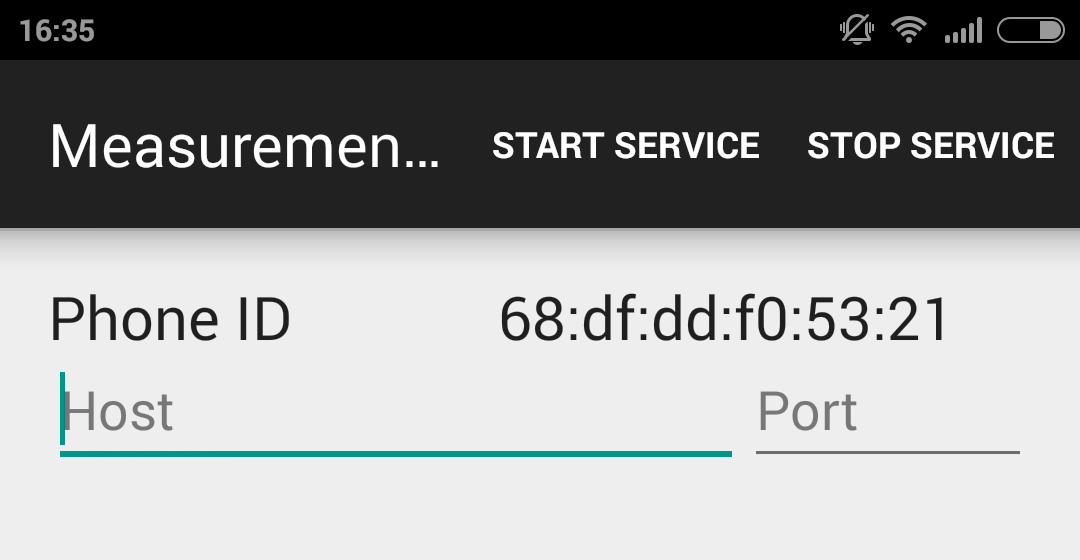
\includegraphics[width=0.25\paperwidth]{figures/measurementapp_activity_crop.png}
		\caption[Android Activity user interface.]{Partial screenshot of the Activity user interface}
		\label{fig:app-activity}
\end{figure}

The Service consists of four separate classes. There is a RecordService that provides the main Service seen by the Android OS. It handles start and stop requests from the Activity or the OS itself, as well as some convenience methods for notifying the user and interacting with the Android user interface. The Service sets itself up as a so-called `foreground service', which implies that it is a purposefully started activity that should take priority over background processes when the system is low on resources.

\paragraph*{}
The bulk of the application is distributed over three threads started by this Service. The NetworkInterfaceThread handles the connection to the \matlab server and loops to receive new messages, as well as sending messages generated by the other threads. As there is only one connection to the server, it was decided to use Java's normal blocking socket system, meaning the thread blocks (and other threads can be run) while no new data has been received.

The NetworkInterfaceThread follows the same state machine described in section \ref{sec:io_fsm} for the \matlab server. When the thread is started, its state is \textsc{setup}. When it has received a packet containing the audio settings for this session, it transmits an acknowledgement packet and changes state to \textsc{idle}. From this point on, it will process a command to start streaming by going into the \textsc{streaming} state, at which point it launches an AudioThread to acquire data from the on-board microphone. During both the \textsc{idle} and \textsc{streaming} states, an OrientationThread is run to acquire orientation data, which is also transferred to the \matlab server.

\paragraph*{}
The AudioThread uses the Android AudioRecord API to initialize the device microphone. As the Android API defines a number of different audio sources meant for different applications \footnote{For more information, see \url{https://developer.android.com/reference/android/media/MediaRecorder.AudioSource.html}.}, it accepts an input argument specifying the audio source to use as a byte. Once the audio source has been successfully initialized, the thread continuously does a blocking read from the audio device into a buffer of its own. Once it has enough samples to transmit a full block (of the length sent by the server), it calls a method in the NetworkInterfaceThread to initiate this transmission. 

\paragraph*{}
The OrientationThread uses the Android SensorManager API to request access to the device magnetometer and accelerometer. The magnetometer produces a vector in the direction of the local magnetic field, and the accelerometer produces a vector in the direction of the so-called `proper acceleration', taking into account the balance of gravitational force and restoration force of the table surface. As such, the magnetometer should produce a vector that points north, and the accelerometer should, at rest, produce a vector that points down.

These vectors are then processed using Android's provided SensorManager.getRotationMatrix to yield a rotation and inclination matrix. These matrices represent the transformation from the device coordinate system (in which the accelerometer and magnetometer measure) to a global coordinate system where X points east, Y points towards magnetic North, and Z points towards the ground. In appendix \ref{app:coordinate_system}, this coordinate system is shown graphically. Finally, the SensorManager.getOrientation method is then called on this matrix to express this transformation in an azimuth, pitch and roll angle that can be sent to the server.

\end{document}
